\section{Projeto}
\sloppy

Esta seção reúne o projeto detalhado da Sprint 4 (Padrões 2), espelhando \path|docs/08-projeto.md| e os ADRs em \path|docs/07-arquitetura/adr/|. Os nomes de classes são os do código, em inglês (ADR-0005).

\subsection{Divisão de pacotes}

As camadas da disciplina (\textbf{ui}, \textbf{business} e \textbf{infra}) correspondem às pastas do aplicativo Next.js. A regra de dependência é \textbf{ui $\rightarrow$ business $\leftarrow$ infra}: a camada business não importa nada de ui nem de infra; cada controle recebe a interface do seu repositório, e a fachada recebe os repositórios pela função passada a \path|getInstance| (ADR-0006, ADR-0007). Telas, Server Actions e rotas de API chamam só a fachada, por \path|getFacade()|.

{\small
\renewcommand{\arraystretch}{1.2}
\begin{longtable}{|p{0.12\textwidth}|p{0.36\textwidth}|p{\dimexpr0.52\textwidth-6\tabcolsep-4\arrayrulewidth\relax}|}
\hline
\textbf{Camada} & \textbf{Pasta} & \textbf{Conteúdo} \\ \hline
\endfirsthead
\hline
\textbf{Camada} & \textbf{Pasta} & \textbf{Conteúdo} \\ \hline
\endhead
ui & \path|src/app/|, \path|src/components/|, \path|src/i18n/| & Telas (inclusive \path|/access-reports|), Server Actions, rotas de API (inclusive \path|GET /api/access-reports|) e textos traduzidos. \\ \hline
business & \path|src/modules/facade/| & \path|FacadeSingletonController| e o tipo \path|Repositories|. \\ \hline
business & \path|src/modules/access-records/| & \path|AccessRecord|, \path|AccessRecordRepository| e erro de persistência. \\ \hline
business & \path|src/modules/access-reports/| & \path|AccessReportTemplate|, \path|HtmlAccessReport| e \path|CsvAccessReport|. \\ \hline
business & \path|src/modules/auth/| & \path|AuthenticationController|, \path|AccessLogger|, permissões por papel e erros de login. \\ \hline
business & \path|src/modules/users/|, \path|src/modules/patients/| & Entidades, regras, erros, interfaces dos repositórios e controles. \\ \hline
infra & \path|src/infra/repository-factory.ts| & \path|RepositoryFactory|, seleção por \path|STORAGE| e família única por processo. \\ \hline
infra & \path|src/infra/in-memory-repository-factory.ts|, \path|src/infra/sqlite-repository-factory.ts| & Famílias de repositórios em RAM e SQLite (conexão compartilhada). \\ \hline
infra & \path|src/infra/users/|, \path|src/infra/patients/|, \path|src/infra/access-records/| & Repositórios RAM e SQLite de cada entidade. \\ \hline
infra & \path|src/infra/logging/| & \path|PinoAccessLogger|, que adapta eventos de autenticação para Pino. \\ \hline
infra & \path|src/infra/facade.ts|, \path|src/infra/auth/|, \path|src/db/| & Montagem da fachada, sessão em cookie assinado, esquema Drizzle (\path|users|, \path|patients|, \path|access_records|) e conexão. \\ \hline
\end{longtable}
}

\subsection{Diagrama de classes de projeto}

O diagrama separa as camadas \textbf{business} e \textbf{infra} para todas as entidades persistidas (\path|User|, \path|Patient| e \path|AccessRecord|). Em business ficam a fachada, os controles, as entidades, as interfaces dos repositórios, o Target \path|AccessLogger| e o Template Method dos relatórios. Em infra ficam a montagem da fachada, a Abstract Factory com as famílias RAM e SQLite, as implementações dos repositórios e o Adapter de log. A biblioteca Pino aparece como pacote externo (Adaptee).

\begin{landscape}
\begin{figure}[H]\centering
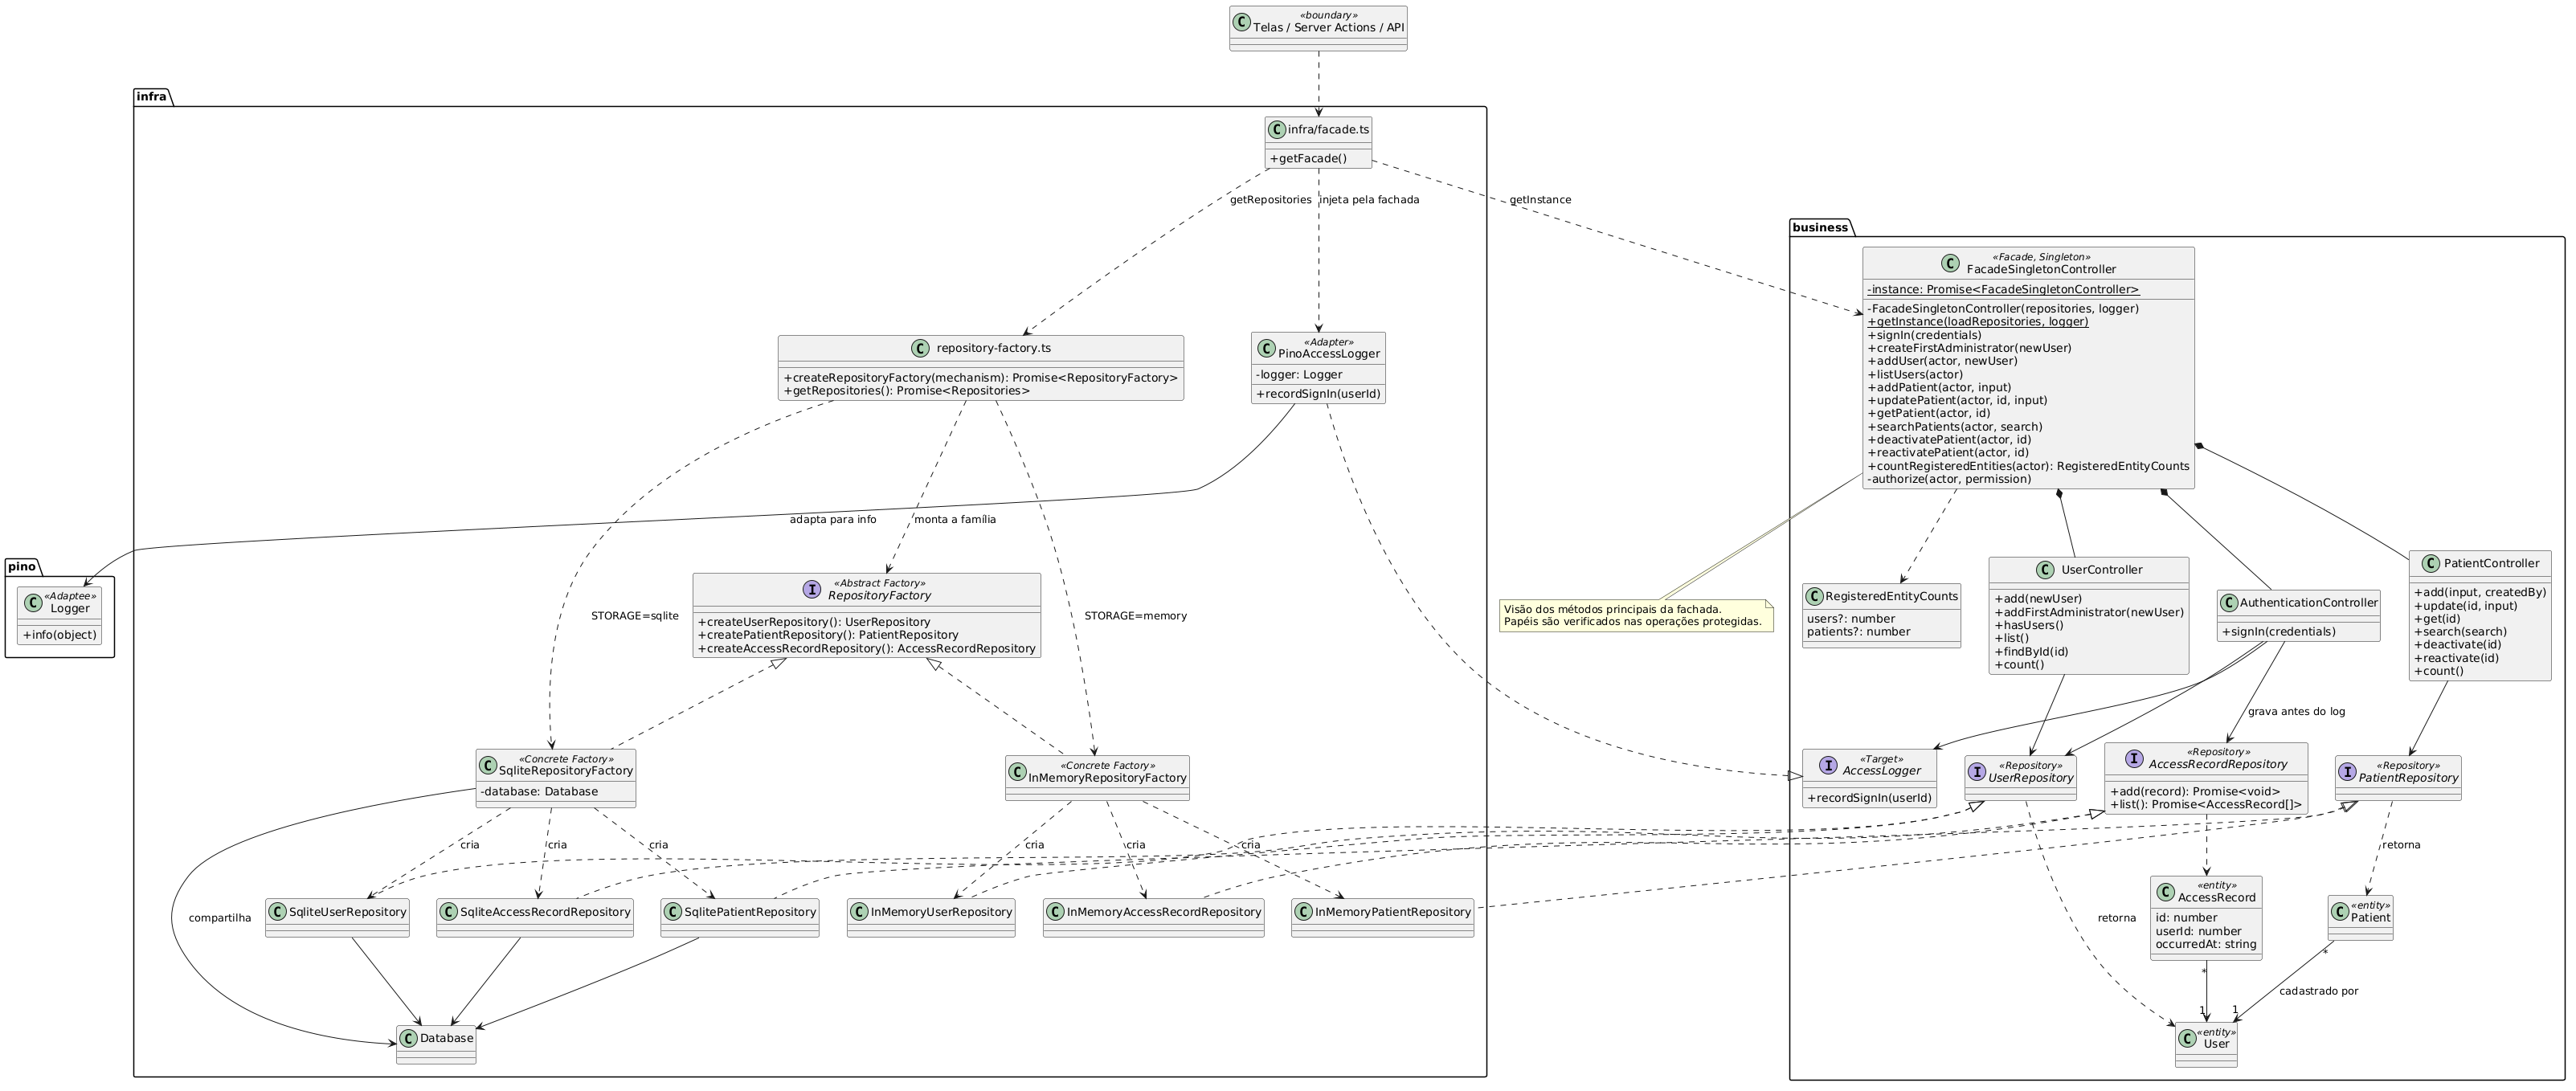
\includegraphics[width=\linewidth,height=0.82\textheight,keepaspectratio]{images/classes-de-projeto.png}
\caption{Classes de projeto da Sprint 4, com as camadas business e infra.}
\end{figure}
\end{landscape}

\subsection{Padrões de projeto aplicados}

\subsubsection{Facade e Singleton (Sprint 3)}

\path|FacadeSingletonController| é o ponto único de entrada da camada business. As fronteiras chamam um só objeto, com um método por caso de uso, e a verificação do papel (NF-SEG-02) fica num só lugar; \path|countRegisteredEntities| informa quantas entidades estão cadastradas. O construtor é privado e a instância fica no campo estático \path|instance|, obtida por \path|getInstance|: os controles e os repositórios são montados uma única vez por processo (ADR-0007). Na Sprint 4, a fachada ganhou \path|generateAccessReport| e passou a receber o logger de autenticação.

\subsubsection{Repository}

\path|UserRepository|, \path|PatientRepository| e \path|AccessRecordRepository| são contratos da camada business. Cada um tem uma implementação em RAM (\path|InMemoryUserRepository|, \path|InMemoryPatientRepository|, \path|InMemoryAccessRecordRepository|) e outra em SQLite (\path|SqliteUserRepository|, \path|SqlitePatientRepository|, \path|SqliteAccessRecordRepository|). Os controles dependem dos contratos, sem conhecer o armazenamento, e as implementações de cada entidade passam pelos mesmos testes de contrato (ADR-0006, ADR-0009).

\subsubsection{Abstract Factory}

\path|RepositoryFactory| é a fábrica abstrata, com \path|createUserRepository|, \path|createPatientRepository| e \path|createAccessRecordRepository|. \path|InMemoryRepositoryFactory| cria a família RAM; \path|SqliteRepositoryFactory| recebe uma conexão e cria os repositórios SQLite sobre ela. \path|createRepositoryFactory| seleciona a fábrica concreta, e \path|getRepositories| lê e valida \path|STORAGE| uma vez e guarda a promessa da família em \path|globalThis|, compartilhada inclusive por chamadas concorrentes. Assim, todas as entidades usam o mesmo mecanismo, o que é necessário porque cada paciente e cada registro de acesso referenciam \path|users| (ADR-0009).

\subsubsection{Adapter}

O Adapter de objeto, por composição, isola a biblioteca de log Pino da camada business:

{\small
\renewcommand{\arraystretch}{1.2}
\begin{longtable}{|p{0.2\textwidth}|p{\dimexpr0.8\textwidth-4\tabcolsep-3\arrayrulewidth\relax}|}
\hline
\textbf{Papel} & \textbf{Participante} \\ \hline
Cliente & \path|AuthenticationController| \\ \hline
Target & \path|AccessLogger|, interface de business com \path|recordSignIn(userId)| \\ \hline
Adapter & \path|PinoAccessLogger|, em \path|src/infra/logging/| \\ \hline
Adaptee & \path|Logger| da biblioteca Pino, método \path|info(object)| \\ \hline
\end{longtable}
}

O Adapter converte \path|recordSignIn(id)| em \path|info({ event: "USER_SIGNED_IN", userId: id })|; Pino acrescenta o horário e escreve JSON em stdout. A montagem em \path|infra/facade.ts| injeta o Adapter na fachada, que o entrega ao controle. O log é operacional e de melhor esforço: exceções síncronas na emissão não impedem uma autenticação válida, e os relatórios não dependem dessa saída (NF-SEG-04, ADR-0010).

\subsubsection{Template Method}

\path|AccessReportTemplate.generate| é o Template Method: valida o período UTC, consulta \path|AccessRecordRepository|, filtra \path|[início, fim)|, agrega por usuário e chama a operação abstrata \path|render|. \path|HtmlAccessReport| e \path|CsvAccessReport| especializam somente a renderização. A contagem inclui registros repetidos, o último acesso é o máximo cronológico, as linhas são ordenadas por ID e o total geral conta todos os registros do período. HTML escapa texto; CSV usa campos entre aspas, escape de aspas e CRLF. Os textos chegam por \path|ReportLabels|, o que permite a tradução na fronteira sem dependência de next-intl em business. Um novo formato implementa \path|render| e reutiliza o mesmo algoritmo (ADR-0011).

\subsection{Tabela de padrões}

{\small
\renewcommand{\arraystretch}{1.2}
\setlength{\tabcolsep}{4pt}
\begin{longtable}{|p{0.13\textwidth}|p{0.08\textwidth}|p{0.34\textwidth}|p{0.27\textwidth}|p{\dimexpr0.18\textwidth-10\tabcolsep-6\arrayrulewidth\relax}|}
\hline
\textbf{Padrão} & \textbf{Sprint} & \textbf{Classes participantes (papel no padrão)} & \textbf{Problema que resolve} & \textbf{ADR} \\ \hline
\endfirsthead
\hline
\textbf{Padrão} & \textbf{Sprint} & \textbf{Classes participantes (papel no padrão)} & \textbf{Problema que resolve} & \textbf{ADR} \\ \hline
\endhead
\raggedright Singleton & S3 & \raggedright \path|FacadeSingletonController| (singleton: construtor privado, campo estático \path|instance|, \path|getInstance|) & \raggedright Os controles e os repositórios são montados uma única vez por processo, e todas as telas e rotas usam a mesma instância & 0007 \tabularnewline \hline
\raggedright Facade & S3 & \raggedright \path|FacadeSingletonController| (fachada); \path|UserController|, \path|AuthenticationController|, \path|PatientController| (subsistema); páginas, Server Actions e rotas de API (clientes) & \raggedright As fronteiras chamam um só objeto, com um método por caso de uso, e a verificação do papel fica num só lugar & 0007 \tabularnewline \hline
\raggedright Repository & S4 & \raggedright \path|UserRepository|, \path|PatientRepository|, \path|AccessRecordRepository| (contratos); implementações \path|InMemory*| e \path|Sqlite*| de cada entidade & \raggedright Os controles dependem dos contratos de negócio, sem conhecer o armazenamento & 0006, 0009 \tabularnewline \hline
\raggedright Abstract Factory & S4 & \raggedright \path|RepositoryFactory| (fábrica abstrata); \path|InMemoryRepositoryFactory|, \path|SqliteRepositoryFactory| (fábricas concretas); os três repositórios (produtos abstratos) & \raggedright Cria uma família de repositórios compatíveis, selecionada uma vez por \path|STORAGE| & 0009 \tabularnewline \hline
\raggedright Adapter & S4 & \raggedright \path|AuthenticationController| (cliente); \path|AccessLogger| (Target); \path|PinoAccessLogger| (Adapter); \path|Logger| do Pino (Adaptee) & \raggedright Traduz eventos de autenticação para log JSON sem acoplar business à biblioteca & 0010 \tabularnewline \hline
\raggedright Template Method & S4 & \raggedright \path|AccessReportTemplate.generate| (Template Method), \path|render| (operação abstrata), \path|HtmlAccessReport| e \path|CsvAccessReport| (subclasses) & \raggedright Reutiliza validação, filtragem e agregação de acessos em formatos diferentes & 0011 \tabularnewline \hline
\end{longtable}
}

Command e Memento estão previstos para a Sprint 5.

\subsection{Decisões de arquitetura da Sprint 4}

\paragraph{ADR-0009: Abstract Factory para a família de repositórios.} As funções independentes de seleção por entidade duplicavam a leitura de \path|STORAGE| e não caracterizavam uma Abstract Factory, e as entidades precisam usar o mesmo mecanismo. Decisão: \path|RepositoryFactory| com as famílias RAM e SQLite, selecionada uma vez por processo. Substitui a seleção independente do ADR-0006. Alternativas descartadas: funções com condicionais, Factory Method por entidade e repositório genérico. Consequência: uma nova entidade persistida exige um método no contrato da fábrica e a implementação nas duas famílias.

\paragraph{ADR-0010: Adapter para log de autenticações com Pino.} Importar uma biblioteca de log no controle acoplaria business à API externa. Decisão: Adapter de objeto, com \path|AccessLogger| em business e \path|PinoAccessLogger| em infra. O contrato recebe somente um ID, impedindo o envio de credenciais ao Adapter. Complemento: o log Pino não é a fonte dos relatórios; \path|AccessRecordRepository| persiste cada acesso antes do log e da sessão, e falhas do banco viram \path|AccessRecordPersistenceError| (API 503, sem sessão).

\paragraph{ADR-0011: Template Method para relatórios de acesso.} \path|AccessReportTemplate.generate| fixa o algoritmo comum e \path|HtmlAccessReport| e \path|CsvAccessReport| especializam \path|render|, evitando divergências estatísticas entre formatos. A fachada verifica \path|GENERATE_ACCESS_REPORTS| (somente ADMIN) antes de validar a entrada ou consultar os dados. Períodos vazios geram total zero; períodos inválidos geram erros específicos por campo; falhas de armazenamento são propagadas. A coleta filtra os registros em memória após \path|list|; consultas por período no banco poderão ser introduzidas caso o volume exija.
